\documentclass[letterpaper,11pt]{article}

%packages
\usepackage{amsfonts}
\usepackage{graphicx}
\usepackage[left=2cm,top=2cm,right=2cm,bottom=2cm,head=.5cm,foot=.5cm]{geometry}
\usepackage{url}
\usepackage{multirow}
\usepackage{longtable}
\usepackage{subfig}
\usepackage{float}
\usepackage{setspace}
\usepackage{lineno}
\usepackage{natbib}
\usepackage{amsmath}
\usepackage{xr}
\usepackage{authblk}
\usepackage{mathrsfs}
\usepackage{relsize}
\usepackage{tikz}

%external documents - this lets you \ref labels defined in the main text, with the prefix MT-.
%The main text does the same thing in reverse, with the prefix SI-, so the two documents can
%cite each other. This works via the .aux file that compiling the other document leaves
%behind, which is why the two documents have to be compiled in alternation (see the
%instructions that accompany this example). 
\externaldocument[MT-]{LatexSimpleExample_Paper}

%The same numeric results that the main text uses, pulled in the same way. See the comment
%in LatexSimpleExample_Paper.tex. 
\newcommand{\outputone}{1.959}
\newcommand{\outputtwo}{0.367}


%header material for paper
\title{A line fitted to ten points: Supporting information}
\date{}

\author[a,b]{Pimsupa Jasmin Albert}
\author[a,*]{Daniel C. Reuman}

\affil[a]{Department of Ecology and Evolutionary Biology and Center for Ecological Research, University of Kansas}
\affil[b]{Environmental Studies Program and Department of Biology, University of Oregon}
\affil[*]{Corresponding author, reuman@ku.edu}

\begin{document}

\linenumbers
\maketitle

\tableofcontents
\listoffigures

\section{Main result reiterated}\label{SIsect:reiter}

%This section is cited from the main text, by its label, with the SI- prefix. And here is how
%the SI cites the main text: the label section:results is defined in the main text. 
The fitted slope of $\hat{\beta}_1=\outputone$ and fitted intercept of $\hat{\beta}_0=\outputtwo$ 
reported in section \ref{MT-section:results} of the main text are truly fundamental. See also 
main-text Fig. \ref{MT-fig:toyline}, which is repeated here as Fig. \ref{fig:toylineSI} for no
good reason except to show that the same results can be included in more than one document. 

\section{Figures}

%The optional argument to \caption, in square brackets, is the short version that goes in the
%list of figures. 
\begin{figure}
\centering
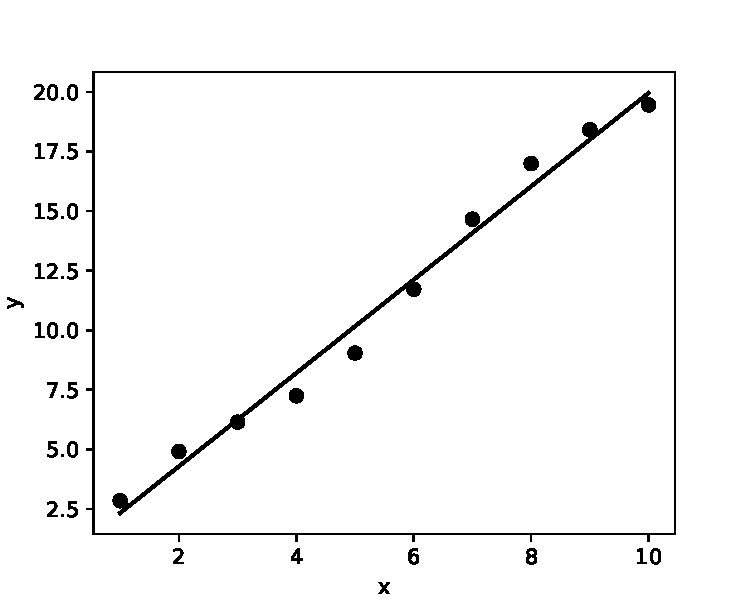
\includegraphics[width=0.6\textwidth]{../results/fig1.pdf}
\caption[The toy data and the fitted line, again]{The ten toy data points (dots) and the line
fitted to them (solid line), slope $\outputone$, intercept $\outputtwo$. This is the same figure
as main-text Fig. \ref{MT-fig:toyline}.}\label{fig:toylineSI}
\end{figure}

\end{document}
